\chapter{Generalities of continuous-wave (CW) radars} \label{cha:generalities}
\chaptermark{Generalities of CW radars}


Continuous-wave (CW) radars are the state-of-the-art technology used in accurate position and velocity measurements of physical media. Of this type of radar systems which transmit and receive continuous radio signals, the most interesting are those which their transmitted signal is modulated in frequency. By linearly modulating the transmitted signal, information about objects having different distances and velocities can be extracted. This radars are known as continuous-wave lineal frequency modulation (CWLFM) radars.

CWLFM radars provide advantages such as robustness to stationary and slow-moving obstacles and clutter, which enable precise measurement of the target of interest. CWLFM radars obtain information on the position and velocity of targets based on the Doppler effect. To understand the advantages of CWLFM radars and its suitableness for the application to the objectives of gait analysis outlined in \cref{cha:intro}, it is of interest to study the basic working principle of these radars and the system requirements necessary to process the information they generate.

\section{CWLFM radars working principle} \label{sec:cwlfm_wp}

The basic working principle of CWFM radars is to obtain a scattered version of a transmitted signal from a target \cite{Ziemer2009}. A modulated signal is transmitted, reaches the target, and reflects back with a frequency variation over time. The beating of the transmitted and received signals contains information about the position and movement of a target.

Typically, linear frequency modulation (LFM) is used for the transmitted signal due to its simplicity. This results in what is known as a CWLFM radar. The transmitted signal can be described with \cref{eqn_st} \cite{Ziemer2009} for $t \in [0, T_c]$ where $\alpha$ is the chirp rate (also called \textit{ramp slope}) defined in \cref{eqn_chirp}, $T_c$ is the repetition interval (also called \textit{ramp time}), $f_0$ is the carrier frequency and $W$ is the swept bandwidth. Therefore the resulting signal is composed of a train of linearly frequency modulated ramps, repeated every $T_c$ seconds \cite{Sardinero2022}. An example of such signal can be seen in \cref{fig_cwlfm_ramps_freq}.
\begin{gather}
	s_T(t) = \cos{\left(2 \pi f_0 t + \pi \alpha t^2\right)} \label{eqn_st}\\
	\alpha = \frac{W}{T_c} \label{eqn_chirp}
\end{gather}

The received signal is a reflection of the transmitted signal by a target at a certain range from the antenna. The received signal is beaten with the transmitted signal to obtain an intermediate frequency (IF) signal. The basic architecture of a CWLFM radar is shown in \cref{fig_cwlfm_arch}. The input of a voltage-controlled oscillator (VCO) is a sawtooth signal with period $T_c$, which in turn creates a signal whose frequency increases linearly with time and repeats every $T_c$ seconds \cite{Sardinero2022}. This signal is amplified and transmitted from an antenna.
\begin{figure}[ht]
	\centering
	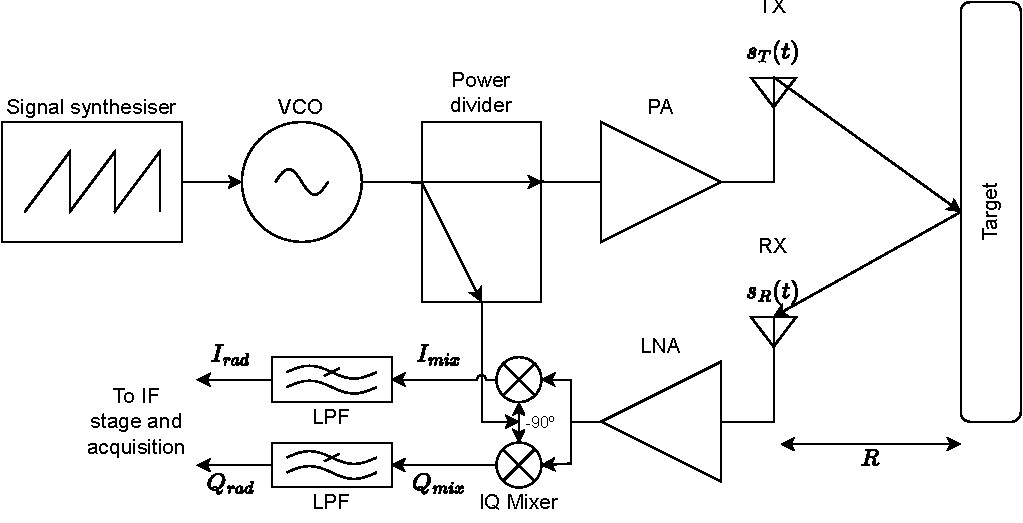
\includegraphics[width=\linewidth]{CWLFM}
	\caption[Basic architecture of a CWLFM radar]{Basic architecture of a CWLFM radar (adapted from \cite{Sardinero2022})}
	\label{fig_cwlfm_arch}
\end{figure}

The transmitted signal is reflected by a target located at a distance $R(\tau_m)$. $\tau_m$ is the \textit{slow time} defined by \cref{eqn_slowtime} where $m$ is each transmission instant \cite{Ziemer2009}. In fact, $\tau_m$ can be seen as a sampled version of $t$. The received signal scattered from such target is defined by equation \cref{eqn_sr} \cite{Ziemer2009,Sardinero2022} where $\sigma$ is the radar cross section (RCS) of the target and $\frac{2R(\tau_m)}{c}$ is the round trip delay. The equation assumes that the target position or movement does not change during each repetition interval $T_c$. An example of a received signal is shown in \cref{fig_cwlfm_ramps_freq}.
\begin{gather}
	\tau_m = t(m T_c); \qquad \forall m \in \mathbb{Z} \label{eqn_slowtime}\\
	s_R(t, \tau_m) = \sqrt{\sigma} \cdot \cos\left[ 2 \pi f_0 \left( t - \frac{2R(\tau_m)}{c}\right) + \pi \alpha \left( t - \frac{2R(\tau_m)}{c}\right)^2 \right] \label{eqn_sr}
\end{gather}

By beating $s_T(t)$ and $s_R(t)$ a beat signal is generated $s_b(t, \tau_m)$. The beat signal contains information in its frequency. The frequency of the beat signal (also called \textit{beat frequency}) $f_b(\tau_m)$ is proportional to the target distance $R(\tau_m)$ as shown in \cref{eqn_fb} \cite{Sardinero2022}. The beat frequency is the difference of the frequencies of the transmitted and received signals. \cref{eqn_fb} holds only at the time intervals where transmitted and received ramps are within the same period \cite{Sardinero2022}. The received signal and the manifestation of the beat frequency as the frequency difference between transmitted and received signals is depicted in \cref{fig_cwlfm_diff}.
\begin{equation} \label{eqn_fb}
	f_b(\tau_m)=\frac{2 \alpha R(\tau_m)}{c} = \frac{2 W R(\tau_m)}{c T_c}
\end{equation}

\begin{figure}[ht]
	\centering
	\subfloat[Frequency variation with time of the transmitted and received signals, where $\Delta t = \frac{2 R(\tau_m)}{c}$]{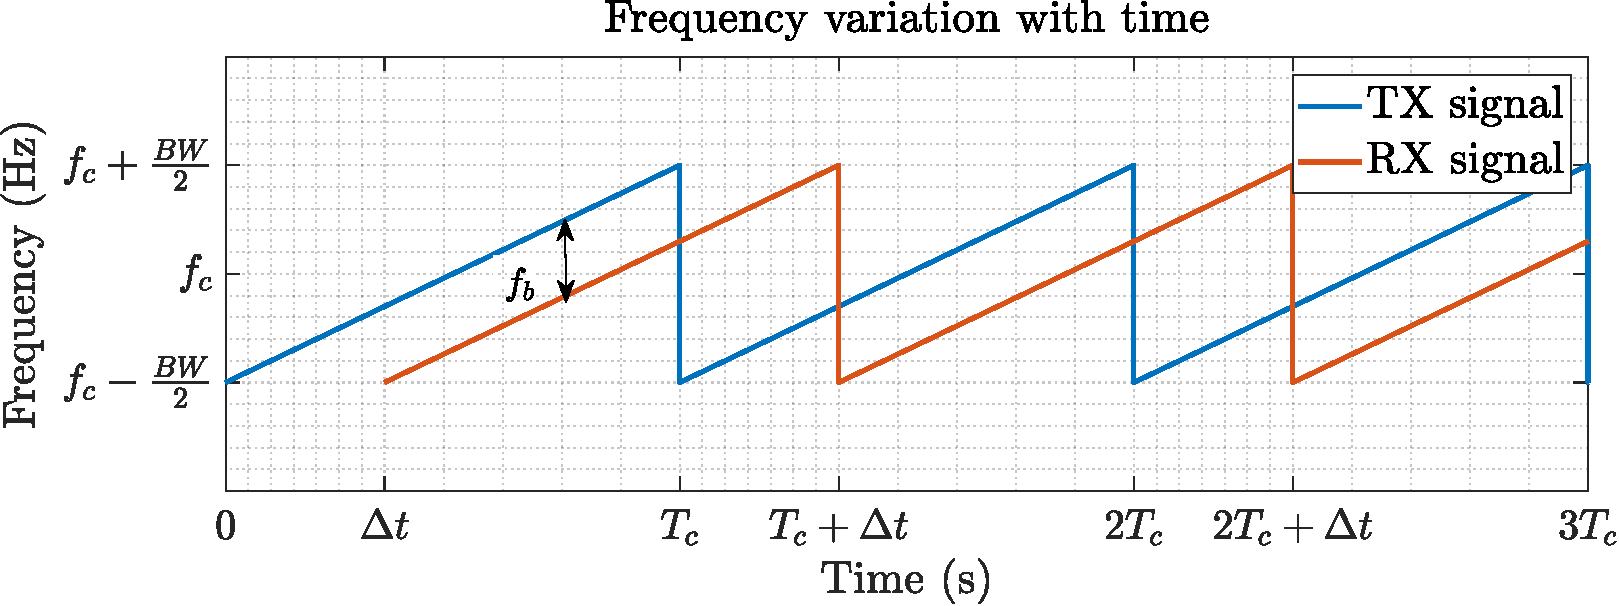
\includegraphics[width=\linewidth]{cwlfm_ramps} \label{fig_cwlfm_ramps_freq}}\\
	\subfloat[Beat frequency variation with time]{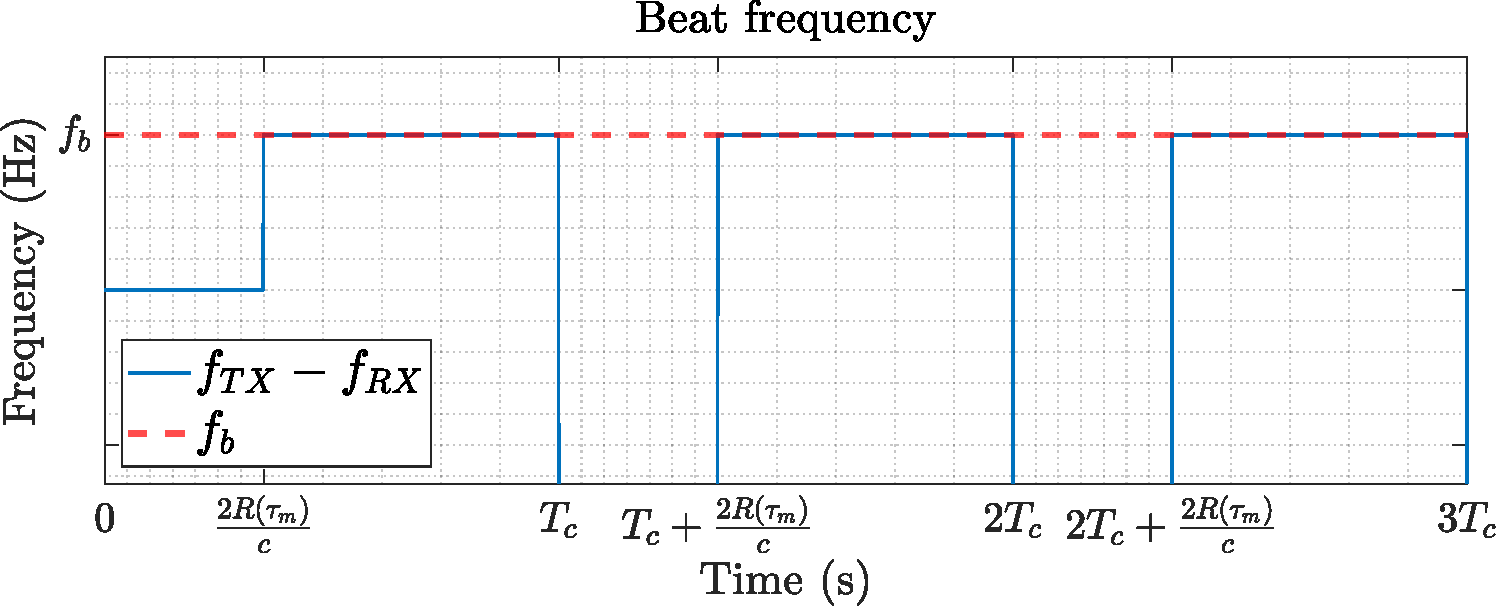
\includegraphics[width=\linewidth]{cwlfm_fb} \label{fig_cwlfm_diff}}
	\caption[Beat frequency for the transmitted and received signal scattered by a target at $R(\tau_m)$ meters away from the radar]{Beat frequency for the transmitted and received signal scattered by a target at $R(\tau_m)$ meters away from the radar. Note that the beat frequency is the difference between frequencies of transmitted an received signals at the time intervals where transmitted and received ramps are within the same period \cite{Sardinero2022} 		\label{fig_cwlfm_ramps}}
\end{figure}

The beat frequency is used for target location, allowing the monitorisation of several people simultaneously \cite{Antolinos2020}. The location can be found by performing the fast Fourier transform (FFT) of the beat signal. The minimum physical separation between to targets so that they can be detected independently (called \textit{range resolution}) can be obtained from \cref{eqn_range_res}, where $W$ is the swept bandwidth and $\sigma \ge 1$ a parameter bound to FFT windowing characteristics \cite{Sardinero2022}.
\begin{equation} \label{eqn_range_res}
	\Delta R = \frac{c}{2W} % TODO: REVISAR \Delta R = \frac{\alpha c}{2W}
\end{equation}

\section{Radar operation} \label{sec:radar_op}

As discussed in \cref{sec:cwlfm_wp}, CWFM radars can be used to obtain the range of a target by measuring the frequency difference between the transmitted and received radar signals. The range of the target is proportional to this frequency difference. To obtain the range measurement, the reflected wave is beaten with the transmitted one. The resulting signal is digitised and processed by an analogue-to-digital converter (ADC). The sampling frequency of the ADC is important in order to avoid valuable information loss.

The Nyquist Theorem \cite{Shannon1949} establishes the relationship between the maximum frequency of the signal and the sampling frequency to avoid information loss:
\begin{equation} \label{eq:nyquist}
	2 f_{\max} \le f_s
\end{equation}
where $f_{\max}$ is the maximum frequency of the output signal.

The maximum range of the radar $(R_{\max})$ determines the maximum frequency of the IF output signal:
\begin{equation}\label{eq:range_max}
	R_{\max} = \frac{f_{\max} c}{2 \alpha} \implies f_{\max} = \frac{2R_{\max} \alpha}{c}
\end{equation}
where $\alpha$ is the slope of the frequency ramp and $c$ is the speed of light.

The slope of the frequency ramp is obtained from \cref{eqn_chirp}, where $W$ is the swept radar bandwidth and $T_c$ is the pulse repetition interval: the time interval between two adjacent ramps.

The pulse repetition interval limits the maximum Doppler frequency ($f_{d\max}$) that can be extracted from the signal:
\begin{equation} \label{eq:doppler_max_tc}
	f_{d\max} = \frac{1}{2 T_c}
\end{equation}

The Doppler frequency $f_d$ is related to the radial velocity of the target $\nu_r$ as follows:
\begin{equation} \label{eq:doppler_max_vr}
	f_d = \frac{2 f_0 \nu_r}{c} \implies f_{d\max} = \frac{2 f_0 \nu_{r\max}}{c}
\end{equation}
where $f_0$ is the central frequency of the radar and $\nu_{r\max}$ is the maximum radial velocity of the target.

By combining \cref{eq:nyquist,eq:range_max,eqn_chirp,eq:doppler_max_tc,eq:doppler_max_vr} the following relationship is obtained:
\begin{equation} \label{eq:fs_final}
	f_s \ge \frac{16 R_{\max}W f_0 \nu_{r\max}}{c^2}
\end{equation}

To enable processing and acquisition of this signal, it is important to use hardware that meets specific requirements.

\section{Hardware requirements for generation and processing of CWLFM signals} \label{sec:general_hw_req}
\sectionmark{Hardware requirements}

As seen in \cref{sec:radar_op}, depending on the variation and range of the magnitudes of interest to be measured, different hardware requirements must be met. In this section, they are detailed the hardware characteristics and parts of the radar system to enable correct processing of the CWLFM radar signals, based on the current CWLFM 24 GHz radar node developed at GMR-SSR \cite{Montesano2019}.

Based on most commercial solutions for CWLFM radars [REF], the radar system which works with CWLFM signals features a baseband stage to control the radiating elements or RF subsystem and an acquisition stage featuring an analogue-to-digital converter (ADC). The acquisition stage is responsible for the digitisation of the CWLFM signals for posterior processing and/or transmission to extract useful information. If the signals from the baseband stage have characteristics that lay outside the working conditions of the ADC, an additional intermediate frequency (IF) stage is necessary to condition these signals. This stage is not present in the current radar node system. A diagram showing the elements present in the currently developed radar node is shown in \cref{fig:system}.

\begin{figure}[ht]
	\centering
	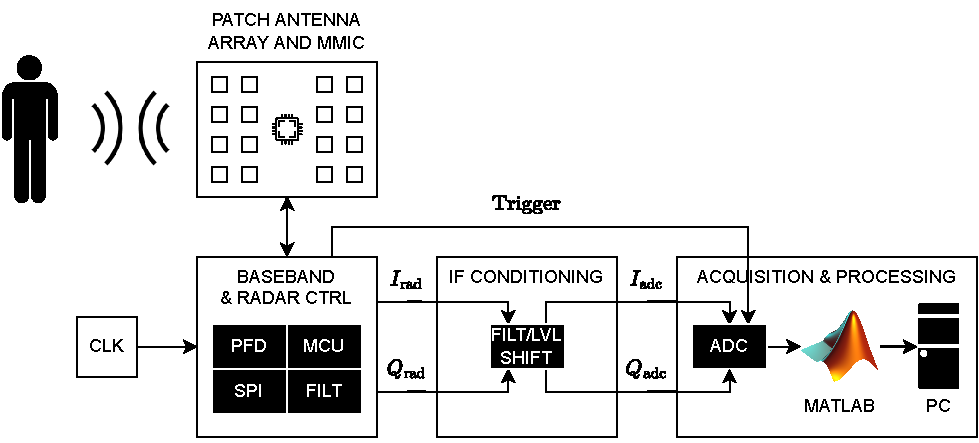
\includegraphics[width=\linewidth]{complete_sys_pc.pdf}
	\caption{Overview of the full radar system components of the currently developed 24 GHz CWLFM radar with corresponding inputs and outputs. Baseband signals are denoted as $I_{\mathrm{rad}}$ and $Q_{\mathrm{rad}}$. Conditioned signals from the IF stage are denoted as $I_{\mathrm{adc}}$ and $Q_{\mathrm{adc}}$ \label{fig:system}} % TODO: change
\end{figure}

\subsection{RF board} \label{sec:rf_board_general}

First and foremost, a printed circuit board (PCB) containing the antennas and the radar element is present. This PCB contains two patch array antennas. One antenna is used for the signal transmission while the other is used for the reception of the rebound signal from the target. The antennas are connected to a microwave integrated circuit (MMIC) from Silicon Radar model TRX-024-046 [REF] which provides an output RF signal for transmission and two intermediate frequency (IF) signals in I and Q format from the reception. The high-level diagram of the MMIC is shown in \cref{fig:block_mmic_general}.

\begin{figure}[ht]
	\centering
	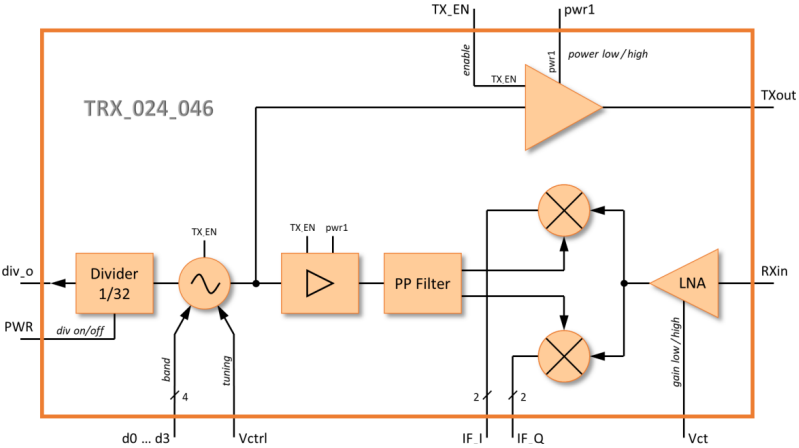
\includegraphics[width=0.8\linewidth]{block_mmic_datasheet.png}
	\caption{High-level diagram of the TRX-024-046 MMIC. The tuning voltage is controlled by the DC level on the \textit{Vctrl} pin and the bandwidth is selected with the \textit{d0...d3} pins. The resulting beating signals are output in the \textit{IF\_I} and \textit{IF\_Q} pins. It is important to note that each pair of IF signals is in differential form \label{fig:block_mmic_general}}
\end{figure}

The signal provided to the transmission antenna is produced by a voltage controlled oscillator, whose bandwidth is configurable and the tuning is provided by a voltage control pin \textit{Vctrl} [REF]. The tuning is controlled by the DC voltage present in the \textit{Vctrl} pin [REF]. This control voltage is generated in an adjacent baseband board described in \cref{sec:baseband_general} connected to this PCB through pinhole conectors. This PCB is manufactured in FR4 dielectric material for the core and is part of the SiRadar EvalKit Easy evaluation kit from Silicon Radar [REF]. An image of the aforementioned PCB with the antennas and MMIC is shown in  \cref{sec:rf_board_general}.

\begin{figure}[ht]
	\centering
	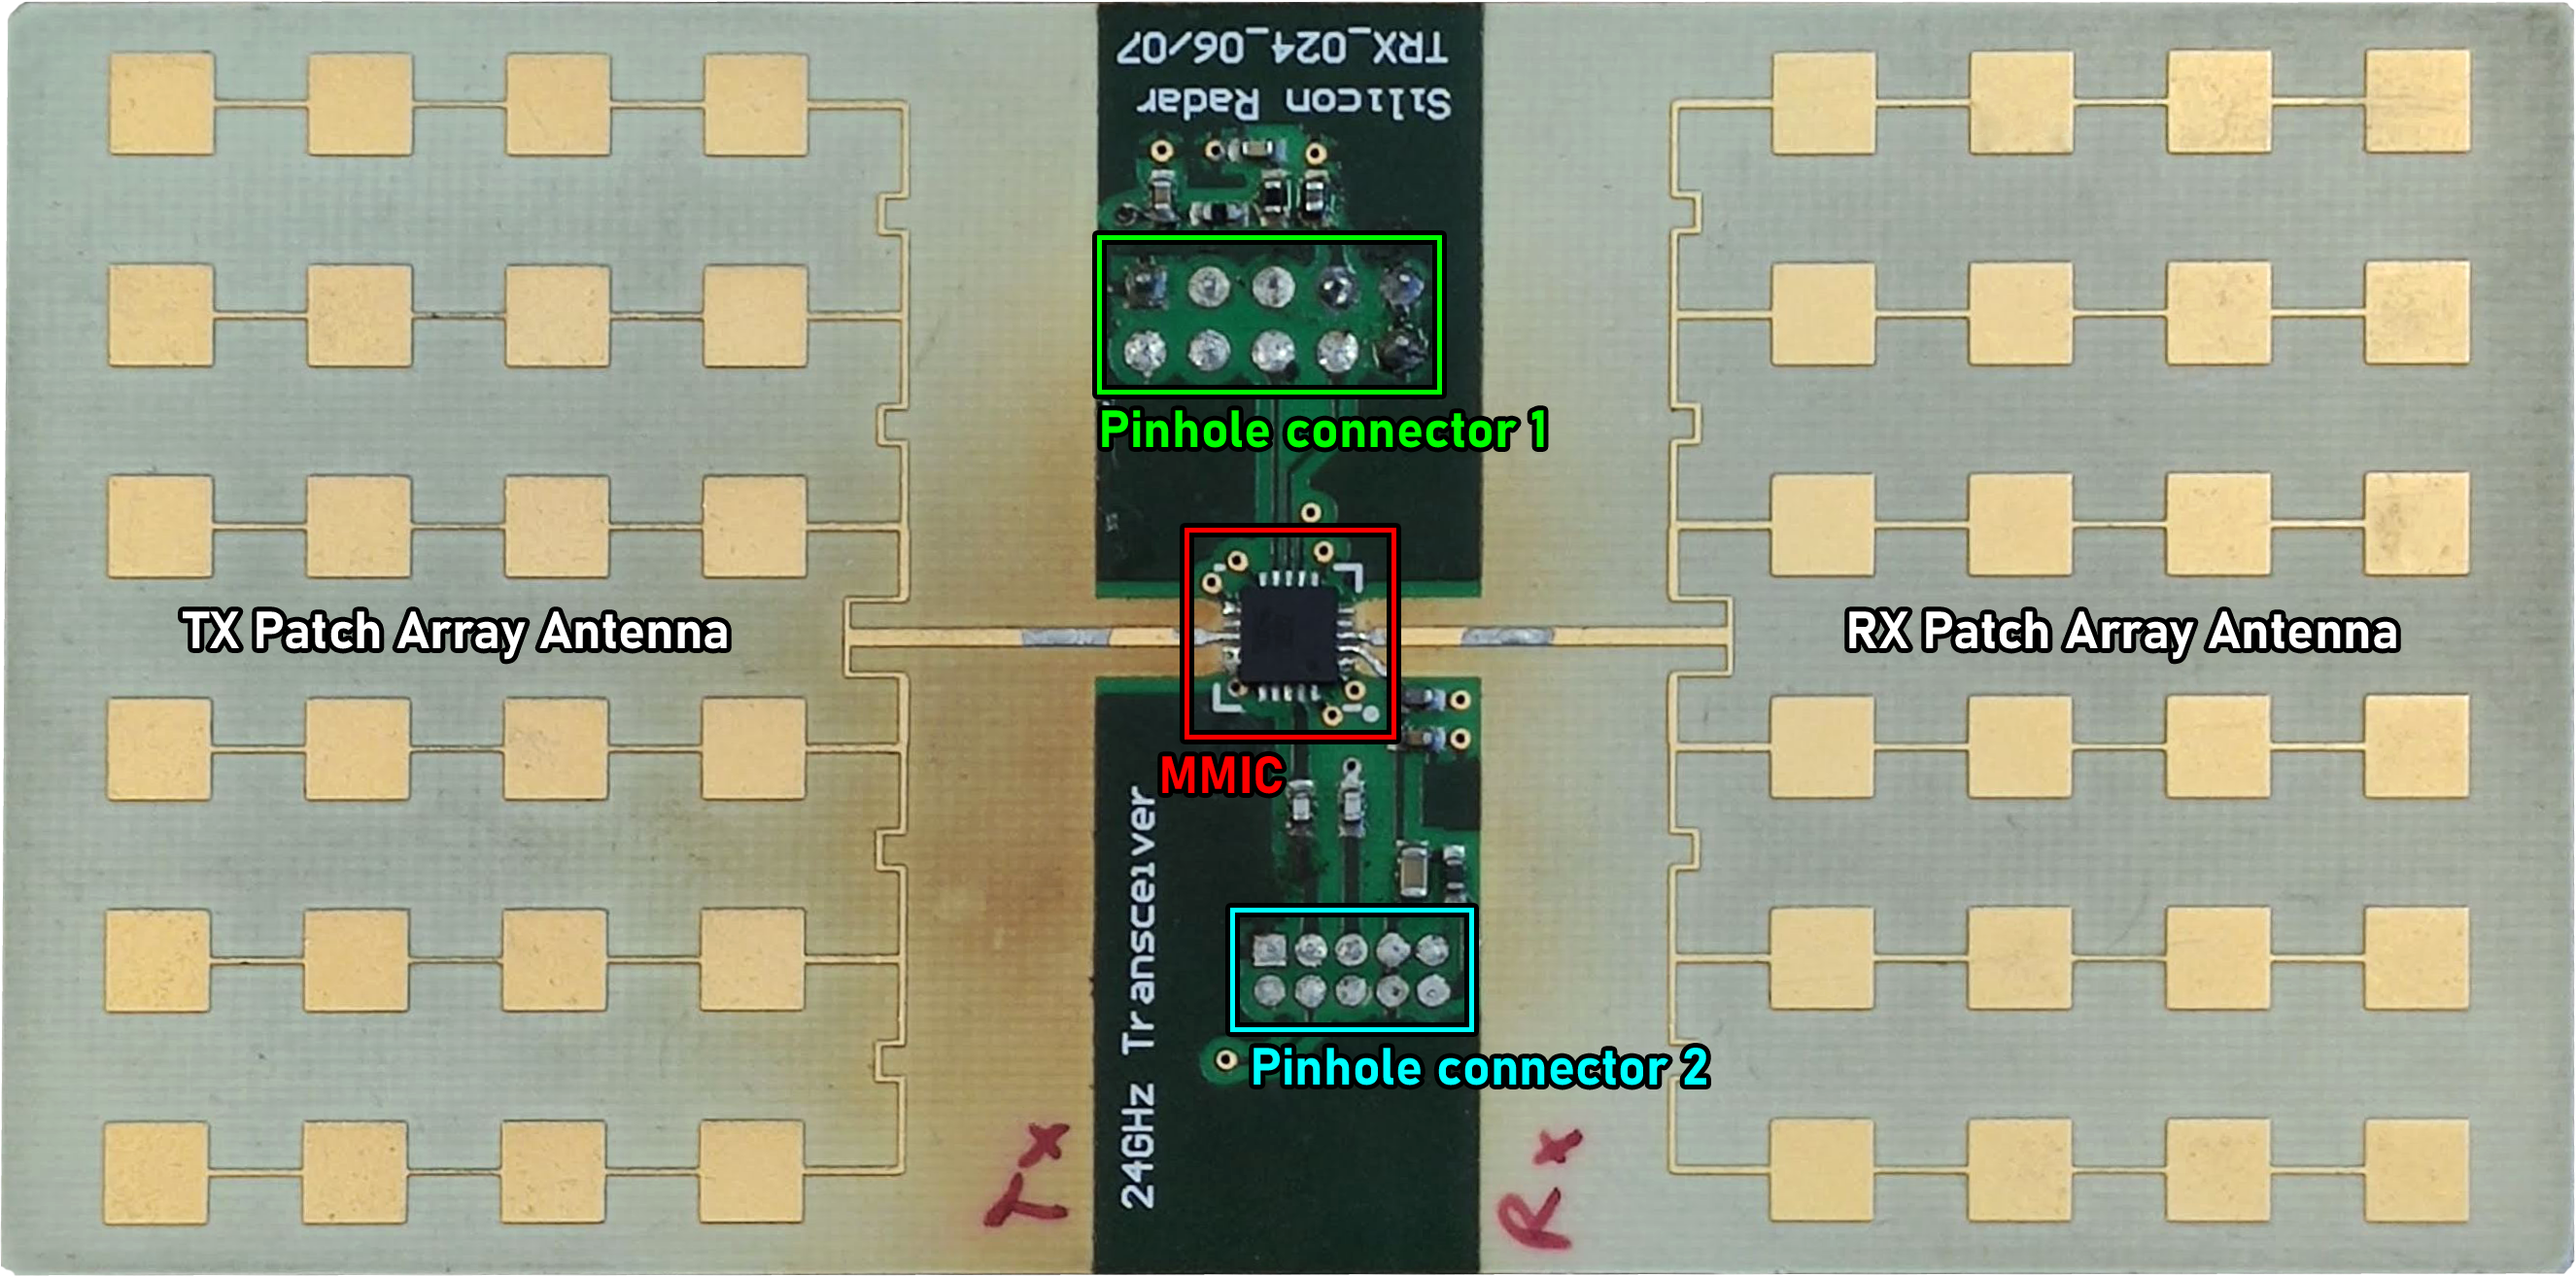
\includegraphics[width=0.8\linewidth]{radar_antenna_mmic.png}
	\caption{Patch antenna and MMIC PCB used in the PCB radar node. The different components are outlined in the image \label{fig:rf_board_general}}
\end{figure}

\subsection{Baseband stage} \label{sec:baseband_general}

The baseband PCB provides the MMIC with the \textit{Vctrl} signal in order to generate the CWLFM ramp signals based on a predefined chirp time and frequency. Additionally, the baseband PCB conditions the IF signals coming from the MMIC. The connection with the RF board is via two pinhole connectors.

This signal is provided by a frequency synthesiser based on a phase frequency detector (PFD), a precision charge pump (CP) and a reference divider. These elements come bundled in a phase-locked loop (PLL) architecture \cite{Sardinero2022}.

The PFD used in the baseband PCB developed at GMR-SSR is from Analog Devices, model ADF4159 [REF DS ZZZ]. The PFD allows configuring parameters such as the bandwidth swept, the ramp or chirp time or the clock source selection through a serial parallel interface (SPI) connection by writing to some specific registers of the PFD integrated circuit (IC) \cite{Sardinero2022, ZZZ}. Therefore, the board also integrates a microcontroller unit (MCU) that is programmed to write to the registers as described in \cite{Sardinero2022}. A detailed description of the PLL architecture of the VCO can be found in Appendix ZZZ.

Finally, the IF signals output by the RF stage are amplified and conditioned to provide a sufficient voltage excursion to enable processing \cite{Sardinero2022}. Therefore amplifying and filtering components are present in this stage. The amplifying and filtering components are described in Appendix ZZZ.

The baseband PCB is manufactured in FR4 dielectric material for the core by the manufacturer Eurocircuits. A high-level diagram of the parts present in the baseband board can be found in \cref{fig:baseband_board_general_diagram}. An image of the manufactured baseband board is found in \cref{fig:baseband_board_general}.

\begin{figure}[ht]
	\centering
	\includegraphics[width=\linewidth, draft]{example-image}
	\caption{High-level diagram of the baseband board elements. The elements depicted are those currently used by the current designed based on \cite{Sardinero2022} \label{fig:baseband_board_general_diagram}}
\end{figure}

\begin{figure}[ht]
	\centering
	\subfloat[Bottom view]{\includegraphics[width=0.5\linewidth]{img/radar_pcb_bot.png} \label{fig:baseband_board_general_bot}}
	\subfloat[Top view]{\includegraphics[width=0.49\linewidth]{img/radar_pcb_top.png} \label{fig:baseband_board_general_top}}
	\caption{Top and bottom views of a manufactured PCB layout of the baseband stage. The elements of this board are outlined by coloured rectangles. Some components are not used in the current radar node design so they are removed. These elements are outlined by grey rectangles. \label{fig:baseband_board_general}}
\end{figure}

%\subsection{Intermediate frequency (IF) stage}
%
%Signals output from the baseband board have a predetermined voltage range and frequency characteristics. Most embedded ADCs have an input range covering only positive voltage values, differing from the input signal peak-to-peak voltage excursion. The I and Q signals output from the baseband board must be conditioned to the ADC voltage input range and the output impedance must be matched to the ADC input impedance.
%
%In many instances, the output signals from the baseband board lack DC level and the baseband stage voltage excursion is not adapted to the ADC voltage range, allowing high discretization errors. Moreover, some MMICs \cite{Antolinos2020} output baseband signals in a differential format. For single-ended ADCs, the signals must be converted to single-ended format.
%% TODO: cambiar cita de elias a una buena
%
%Nonetheless, this stage is not necessary provided that the ADC input voltage range can be adjusted and fitted to the baseband signals voltage excursion and the output configuration matches the input configuration of the ADC.
%
%Should it be necessary to condition the signal, an intermediate frequency (IF) stage is used. The IF stage provides gain and DC shifting to the input signals for correct digitisation. To that effect, the IF stage must have the following capabilities:
%\begin{itemize}
%	\item Conversion from differential to single-ended signal configurations (bypassable)
%	\item Linear, low-noise amplification, filtering and DC shifting
%\end{itemize}
%
%A high-level overview of the architecture for this stage is shown in \cref{fig:if_general}. This stage can be laid out in a separate board to prioritise modularity or integrated with other stages in a single board to favour compactness and power efficiency.
%
%\begin{figure}[ht]
%	\centering
%	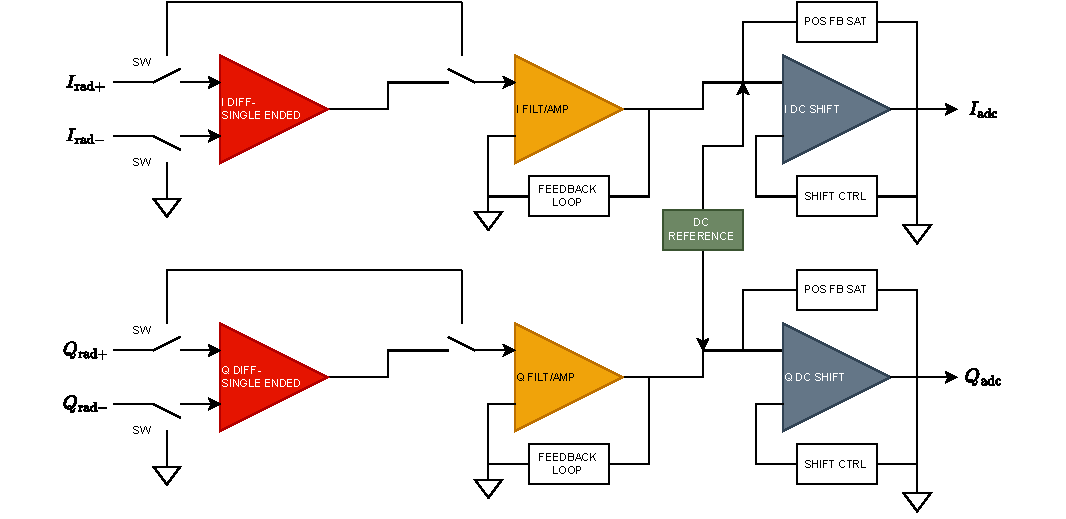
\includegraphics[width=\linewidth]{if_stage_diagram.pdf}
%	\caption{High-level architecture of the intermediate frequency (IF) stage for signal conditioning and impedance matching \label{fig:if_general}}
%\end{figure}

\subsection{Acquisition stage}

In the current design, the IF signals from the baseband board are driven directly to the acquisition stage. Conversion of the filtered and conditioned signals from the analogue domain to a digital representation is carried out in this stage. The current implementation feature an acquisition stage composed of an ADC connected to a PC, which follows the current commercial and state-of-the-art implementations [REF]. This setup allows for post-processing the captured signals on the PC.

To subsequently achieve a correct sampling of the signals, the ADC must be able to sample at a rate higher than the minimum sample rate $f_s$ as per \cref{eq:fs_final}, which is dependant of the Nyquist criteria outlined in \cref{eq:nyquist} and the Doppler range-frequency characteristic shown in \cref{eq:doppler_max_vr}. These characteristics vary depending on the application, for instance, they rely on the maximum Doppler velocity to be measured. Ensuring correct acquisition in a wide variety of scenarios can only be achieved by selecting an ADC with a sufficiently high $f_{s_{\max}}$.

\cref{fig:adc_general} shows a high-level diagram describing the hardware present in the acquisition stage. Signals from the baseband stage ---or conditioned with an IF stage--- must be sampled and processed accordingly. The general processing pipeline features a digitiser card connected to a PC via a high-speed port (such as Peripheral Component Interconnect (PCI)). The ADC card is instructed by a control program to sample for a predetermined amount of time at a particular sampling frequency. After collecting the samples and storing them on the on board memory of the ADC, they are transferred to the random access memory (RAM) of the computer to be accessed by a digital signal processing (DSP) software such as MATLAB. It is important to note that the sampling and processing is done in a deferred way, as the DSP takes place after the measurement capture process finishes \cite[p.~43-44]{ADLINKTechnologies2010}. The implementation of the radar node available at GMR makes use of the ADLINK Technologies PCI-9846 ADC card.

\begin{figure}[ht]
	\centering
	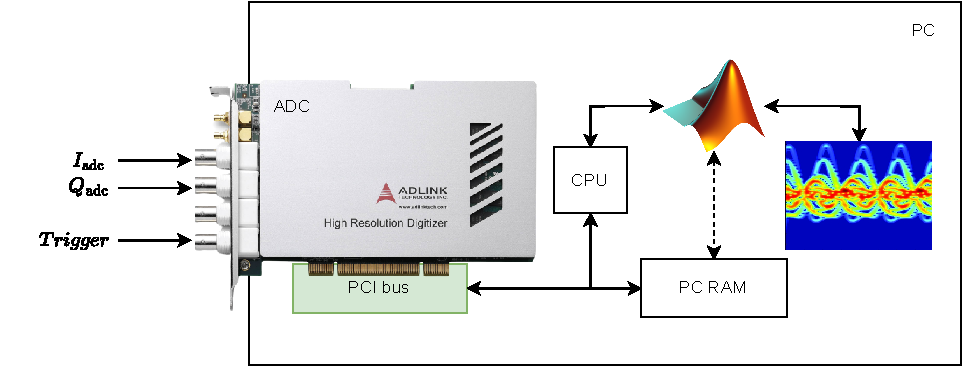
\includegraphics[width=\linewidth]{adc_stage_pc_diagram.pdf}
	\caption{High-level architecture of the acquisition stage for signal digitisation \label{fig:adc_general}}
\end{figure}


\section{Hardware cost}

The different stages described in \cref{sec:general_hw_req} are composed of a set of materials and hardware components that form the complete system of one radar node. It is of interest to analyse the final cost of manufacturing one radar node.

State-of-the-art commercial implementations follow the general requirements outlined in \cref{sec:general_hw_req}. A specific implementation has been developed at GMR that features the general stages present on a CWLFM radar node \cite{Sardinero2022}. For this implementation, the cost per unit of a single radar node has been analysed at the time of writing. A summarised overview of the cost per part of the system is shown in \cref{tab:cost_stages}. The detailed cost per component for a single node is outlined in Appendix ZZZ.

Firstly, it can be seen that the IF stage cost, even when necessary, is negligible compared to the total cost of the node, thus its analysis is not of interest. The baseband stage contributes minimally to the overall cost, despite being priced more than one order of magnitude than the IF stage. Nonetheless, the most expensive stage by far is the acquisition stage. In fact, this stage contributes to almost the entirety of the cost of the system. Conclusively, a radar node costing almost as much as the cost of the its acquisition stage is not a figure of merit of the system.

\begin{table}
	\centering
	\begin{tblr}{
			width = \linewidth,
			colspec = {X[2.5,l]
				X[2,si={table-format=3.2,table-number-alignment=right},r]
				X[4,si={table-format=3.2,table-number-alignment=right},r]},
			row{1,Z} = {font=\bfseries},
		}
		\toprule
		{{{Stage}}} & {{{Subtotal (EUR)}}} & {{{Contribution to total cost (\%)}}}\\
		\midrule
		Baseband stage & 367.79 & 6.38 \\
		IF stage & 21.34 & 0.37 \\
		Acquisition stage & 5380.00 & 93.25 \\
		\midrule
		Total cost & 5769.13  & 100.00 \\
		\bottomrule
	\end{tblr}
	\caption{Cost breakdown of a radar node following the general design}
	\label{tab:cost_stages}
\end{table}

\begin{table}
	\centering
	\begin{tblr}{
			width = \linewidth,
			colspec = {X[l,h]
				X[si={table-format=3.2,table-number-alignment=right},r]
				X[si={table-format=3.2,table-number-alignment=right},r]
				X[si={table-format=3.2,table-number-alignment=right},r]
				X[si={table-format=3.2,table-number-alignment=right},r]},
			row{1,Z} = {font=\bfseries},
			row{1} = {guard},
		}
		\toprule
		Item & Units & Cost/unit (EUR) & Item cost (EUR) & Contrib. to total cost (\%)\\
		\midrule
		PC & 1 & 950.00 & 950.00 & 16.47 \\
		Annual MATLAB License & 1 & 800.00 & 800.00 & 13.87 \\
		ADC (ADLINK PCI-9846) & 1 & 3630.00 & 3630.00 & 62.92 \\
		\midrule
		Subtotal cost & & & 5380.00 & 100.00 \\
		\bottomrule
	\end{tblr}
	\caption{Cost breakdown of the acquisition stage of a radar node following the general design}
	\label{tab:cost_acquisition}
\end{table}

To understand the high cost of the acquisition stage, it is of interest to study the parts included in the general design of this stage \cite{Sardinero2022}. \cref{tab:cost_acquisition} shows the cost of the different parts comprising the acquisition stage of the general design. It is shown that the ADC itself assumes more than half the cost of a single radar node. Additionally, other high costs of the stage cannot be neglected. Those costs are related with the equipment and software necessary to interface with ADC. This is currently achieved with a PC executing the MATLAB software to extract data from readings of the ADC and later process the samples accordingly. Thus, a sufficiently fast PC and a MATLAB license are required as well.

For the objective of developing multi-static radar networks, a high cost per node entails difficulties in scaling up the number of nodes to be manufactured and integrated into a system. Furthermore, the need to use a PC to obtain and process the samples poses a problem for the portability, energy efficiency and compactness of the nodes, making it difficult to integrate them in closed spaces.

In conclusion, the current state-of-the-art acquisition and processing stage and pipeline severely increases the cost of the radar nodes. In the context of the use of radar networks for gait analysis, radar nodes must be cost-effective and compact.

% adc does batch / deferred processing instead of real-time continuous processing.